\section{Optimization}
% area and performance estimation
% design space
% optimization : 3 trade-off


The evaluation of a circuit is through its used area and performance. This aspect can be only optimized during the architectural synthesis. So it is important to have the ability to estimate the area used and resulted performance. This then used to make further optimization until the optimum circuit can be produce. The area and performance estimation and optimization during high level synthesis can be done during sharing and binding process. This is due to the fact that a binding provide the information about the area of a circuit and schedule provide the latency with given cycle-time. In this section, we will go through the step in estimating area and performance of a circuit. Then we will go further with the optimization strategies.



\subsection{Area and performance estimation}

In general circuit, the total area of a circuit is the sum of area of resource, steering logic, register, control unit and wiring area. The number of those component used in a circuit is depends on binding as well as schedule. Reducing the number of used resource linearly does not mean that area is reduced linearly. As we discussed in pervious section, resource sharing is applied to reduce used area and reducing the number of resource also cause the increasing number of steering logic, register and control unit. That means the number of every single component affect the used area.

Circuit performance can be evaluated through circuit schedule. As we discussed before in pervious section, schedule sequencing graph provide us the value of latency, $\lambda$ , propagation delay of an operation and cycle-time. Since the value of latency with defined cycle-time affected by binding, that give us information about maximum number of operation with the same type can run concurrently, we can also estimate the performance through binding. Binding explicitly describe the type and number of component being used. That means every single component affect the performance because the number of resource affect the total of propagation delay and latency.

So it is important to know how the number of every single component such as resource, steering logic, wiring and control unit affect the area and performance. The list below explain how The components affect the area and performance \cite{main}.

\begin{itemize}
    \item Resource : A resource affect the area and performance through its size and its propagation delays of combinational logic.
    \item Steering logic : Steering logic affect the propagation delay of a resource. The effected area can be estimated depend on the number of input and out put of a multiplexer used as we discuss in pervious section. 
    \item wiring : Wiring contribute to overall area and delay. Estimating the wiring area and length requires the knowledge of the structure. The delay cause by wiring can be estimated through its length.
    \item Control unit : Control unit contribute to overall area and delay. The area of control unit can be estimate based on latency because the word length used to accommodate all control step can be estimated.
\end{itemize}

Next, which is the last step in our synthesizing process will be discussed, which is optimization strategies.

\subsection{Optimization strategies}

In this subsection, we will discuss circuit optimization. Optimization process involve scheduling and binding in order to optimize the area, latency and cycle-time because of the aim of architectural optimization is to find a scheduled sequencing graph with a complete resource binding that met all the given constraints \cite{main}. An optimum circuit can be built if the circuit is not influenced only by one aspect, e.g. area, but fairly influenced by all aspect. As explained in pervious section, particularly in compatibility graph subsection, we can see that reducing number of resource cause more operation need to share some resource, thus the operation cannot run concurrently, and the latency need to be increased. On the other hand, increasing the number of resource could reduce the latency but increase the total area of a circuit. Reducing the cycle time could cause an operation to take two cycles to complete. All the possibilities can be structure in design evaluation space. To have an optimum circuit, we need to find a point where all aspects are fairly dominate the circuit. This point is called Pareto point \cite{main}.


To have this point, a designer should traverse the design evaluation space. Architectural exploration is often done by exploring the (area/latency) trade-off for different values of the cycle-time \cite{main}. Another approach is through search for the (cycle-time/latency) tradeoff for some binding or the (area/cycle-time) trade-off for some schedules.

Next we will go through for each design evaluation space.

\subsection{(area/latency) trade-off}

In (area/latency) trade-off design evaluation space, the value of cycle time is fixed. The extreme point of each aspect, area and latency, can be found by finding the minimum value of latency and resource accordingly. The design evaluation space can be explored by reducing one parameter as a function of the other. 

Based on our circuit model as in ``Fig. \ref{scheduled_sequencing_graph}", we make assumption as below : 
\begin{itemize}
    \item Area constraint is 20 units.
    \item Latency less than 8 cycles.
    \item ALU propagation delay is 25 ns.
    \item Multiplier propagation delay is 35 ns.
\end{itemize}

Since the cycle time should be fixed, if we set the cycle-time to 40ns, every operation will take one cycle time, but if we set it to 30ns, multiplier will take two cycles to complete. Now we fix our cycle time to 40ns.

If we took only one multiplier, the resulting latency is 13, and it will break the constraint. if we choose two multiplier and one adder, the resulting latency and area is 8 cycles and 12 unit. The exploration can be continued by trying all the possibilities as shown in ``Fig. \ref{Design_evaluation_space_area_latency_Trade_off_points_for_two_values_of_the_cycle-rime}".

\begin{figure}[ht]
    \centering
    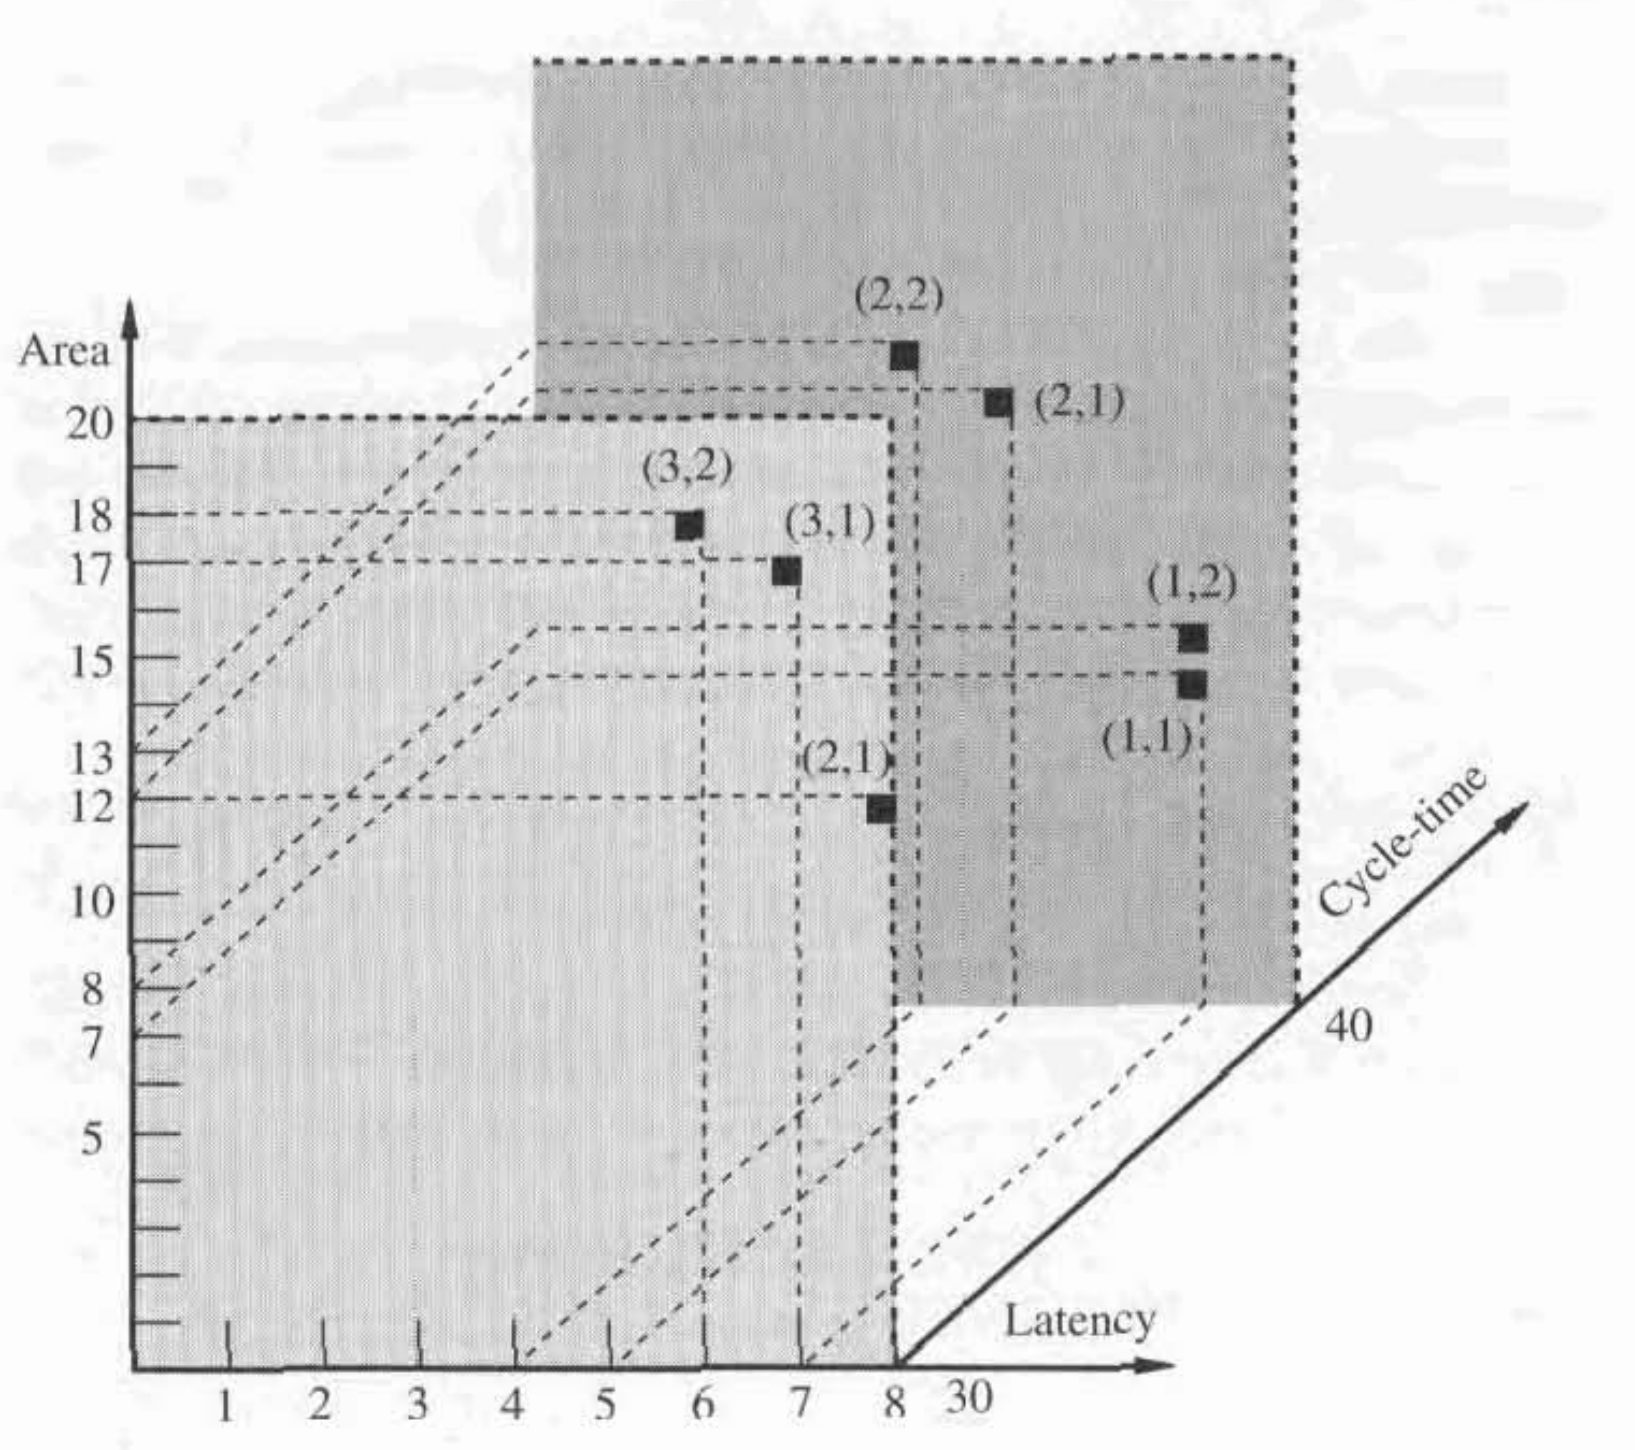
\includegraphics[width=0.4\textwidth]{Design_evaluation_space_area_latency_Trade_off_points_for_two_values_of_the_cycle-rime}
    \caption{Design evaluation space: area/latency trade off points for two values of the cycle time. \cite{main}}
    \label{Design_evaluation_space_area_latency_Trade_off_points_for_two_values_of_the_cycle-rime}
\end{figure}


\subsection{(cycle-time/latency) trade-off}

By fixing the value of total area, we could try to draw a possible point by changing the value of number of component and see how the value of cycle-time and latency affect each other as shown in ``Fig.\ref{Design_evaluation_space_some_cycle_timenatency_trade-off_points_for_two_bindings}". From our discussion in the pervious section, the method that used weighted compatibility graph could be helpful.  

\begin{figure}[ht]
    \centering
    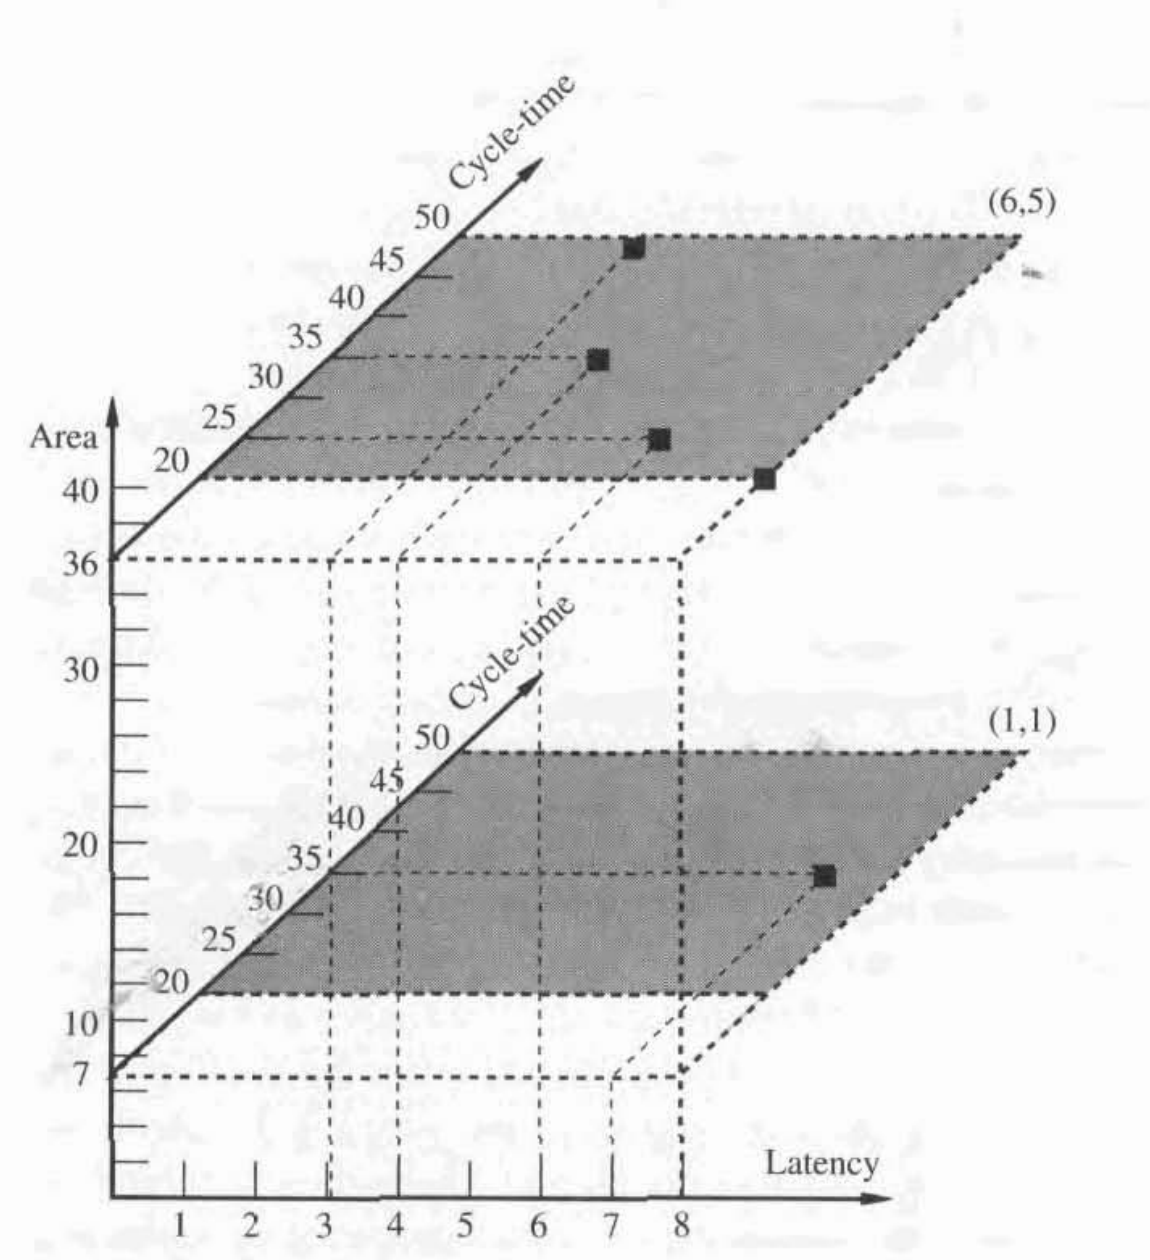
\includegraphics[width=0.4\textwidth]{Design_evaluation_space_some_cycle_timenatency_trade-off_points_for_two_bindings}
    \caption{Design evaluation space: cycle-time/latency trade off points for two values of the area. \cite{main}}
    \label{Design_evaluation_space_some_cycle_timenatency_trade-off_points_for_two_bindings}
\end{figure}


\subsection{(area/cycle-time) trade-off}

By fixing the value of latency, we could try to draw a possible point by changing the value of number of component and see how the value of cycle-time and area affect each other as shown in ``Fig.\ref{Desisn_evilluatinn_apace_some_cycle_timellarcncytmde_of_points_far_wo}" by applying possible methods from pervious section.

\begin{figure}[ht]
    \centering
    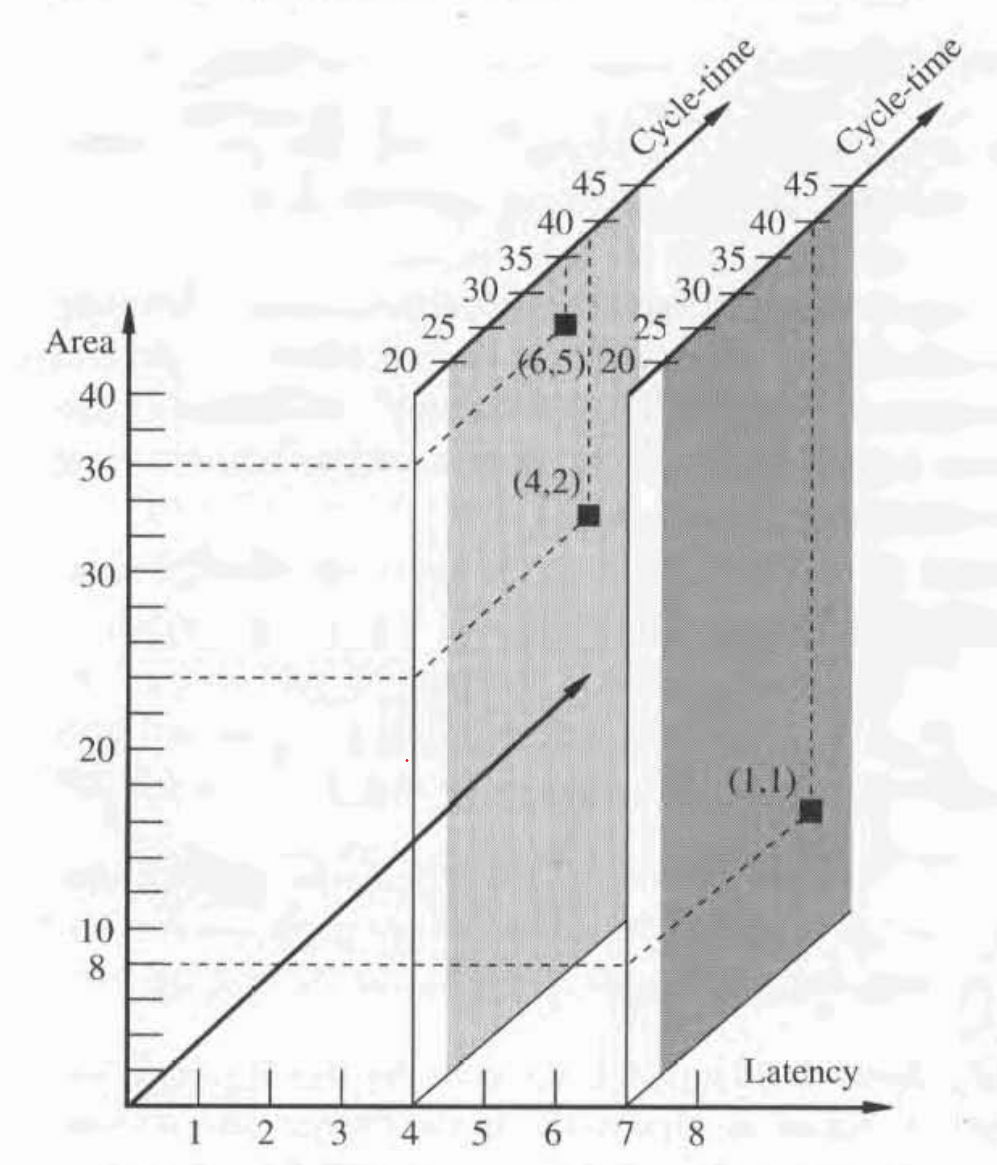
\includegraphics[width=0.4\textwidth]{Desisn_evilluatinn_apace_some_cycle_timellarcncytmde_of_points_far_wo}
    \caption{Design evaluation space: area/cycle-time trade off points for two values of the latency. \cite{main}}
    \label{Desisn_evilluatinn_apace_some_cycle_timellarcncytmde_of_points_far_wo}
\end{figure}


